%%%%%%%%%%%%%%%%%%%%%%%%%%%%%%%%%%%%%%%%%
% Friggeri Resume/CV
% XeLaTeX Template
% Version 1.2 (3/5/15)
%
% This template has been downloaded from:
% http://www.LaTeXTemplates.com
%
% Original author:
% Adrien Friggeri (adrien@friggeri.net)
% https://github.com/afriggeri/CV
%
% License:
% CC BY-NC-SA 3.0 (http://creativecommons.org/licenses/by-nc-sa/3.0/)
%
% Important notes:
% This template needs to be compiled with XeLaTeX and the bibliography, if used,
% needs to be compiled with biber rather than bibtex.
%
%%%%%%%%%%%%%%%%%%%%%%%%%%%%%%%%%%%%%%%%%

\documentclass[]{scoggins-cv} % Add 'print' as an option into the square bracket to remove colors from this template for printing

\usepackage{fontspec}
\newfontfamily{\FA}[Path = fonts/]{fontawesome-webfont}

\usepackage{ragged2e}

\usepackage{marginnote}
\usepackage{geometry}
\geometry{
  verbose,
  tmargin=2.5cm,
  bmargin=2cm,
  lmargin=5.2cm,
  rmargin=2.5cm
}
\def\faEnvelope{{\FA\symbol{"F0E0}}}
\def\faGithub{{\FA\symbol{"F09B}}}
\def\faDesktop{{\FA\symbol{"F108}}}
\def\faPhone{{\FA\symbol{"F095}}}
\def\faHandPointerO{{\FA\symbol{"F25A}}}
\def\faMapMarker{{\FA\symbol{"F041}}}
\def\faVideoCamera{{\FA\symbol{"F03D}}}
\def\faCloudDownload{{\FA\symbol{"F0ED}}}

\input{citationskip}

\begin{document}

\header
\section{Matthew T. Scoggins}
%----------------------------------------------------------------------------------------
%	Contact
%----------------------------------------------------------------------------------------
%\iffalse
\aside{Contact}{-.5035}{
    %
    \vspace*{-0.1cm}
    %
    %
    \href{https://github.com/mscoggs}{{\addfontfeature{Color=linkblue}github.com/mscoggs}\ \faGithub}\\[0.5em]
    %
    \href{mscoggs.github.io}{{\addfontfeature{Color=linkblue}mscoggs.github.io}\ \faHandPointerO}\\[0.5em]
    %
    \href{tel:360-325-3398}{{\addfontfeature{Color=linkblue}+1 (360) 325 3398}\ \faPhone}\\[0.5em]
    \href{mailto:mts2188@columbia.edu}{{\addfontfeature{Color=linkblue}mts2188@columbia.edu}\ \faEnvelope}\\[.01em]
    %
    %\href{https://www.astro.columbia.edu/content/matthew-scoggins}{{\addfontfeature{Color=linkblue}\small Astronomy Department }\\
    %    \href{https://www.astro.columbia.edu/content/matthew-scoggins}{{\addfontfeature{Color=linkblue}\small Columbia University}}\ \faMapMarker}
    %
}
%\fi
%----------------------------------------------------------------------------------------
%	EDUCATION
%----------------------------------------------------------------------------------------
\vspace{-0.5cm}
\section{Education}
\vspace{-0.3cm}

\begin{entrylist}

    %------------------------------------------------

	\vspace{-0.3cm}
    \entry
    {2021--}
    {PhD {\normalfont Astrophysics}}
    {Columbia University, New York, NY}
	{}


    %------------------------------------------------

    \entry
    {2015--2020}
    {BS {\normalfont Physics, Math,} BA {\normalfont Philosophy}}
    {Western Washington University, Bellingham WA}
	{}
    %------------------------------------------------
\iffalse
    \entry
    {2013-2015}
    {AS}
    {Whatcom Community College, Bellingham WA}
\fi
    %------------------------------------------------

\end{entrylist}

\vspace{-0.3cm}
%----------------------------------------------------------------------------------------
%	ABOUT
%----------------------------------------------------------------------------------------
%\vspace{-0.8cm}
%\iffalse

\aside{About Me}{2.035}{
    \footnotesize
    I am a third-year PhD Student in the Department of Astronomy at Columbia.
    My research interests span most areas of computational astrophysics and cosmology.
    Specifically, I am interested in questions involving supermassive black holes, the early universe, and Population III stars.
}
%\fi
%----------------------------------------------------------------------------------------
%	POSITIONS
%----------------------------------------------------------------------------------------
\section{Positions}

\begin{entrylist}
    \entry
    {2021--}
    {Graduate Researcher}
    {Columbia University, New York, NY}
    {%
        \vspace{-1em}
        \begin{list}{{\color{numcolor}$-$}}{\cvlist}
	  \item Supermassive star formation and their role in seeding supermassive black holes
          \item Learning the Universe: Using machine learning to accelerate forward modeling of cosmological simulations
          \item Observable consequences of the heavy seed origin for supermassive black holes
          \item SETI: Numerical investigations of star-lifting, identifying observable features of star-lifting

          \item Advised by Zoltan Haiman, Greg Bryan, David Kipping
        \end{list}
    }
    %------------------------------------------------


  \entry
  {2021-2023}
  {Graduate Teaching Assistant}
  {Columbia University, New York, NY}
  {%
      \vspace{-1em}
      \begin{list}{{\color{numcolor}$-$}}{\cvlist}
        \item Spring 2023: TA for Astro I Lab
        \item Fall 2022: Observational TA for Astro I Lab
        \item Spring 2022: Astrophysics II for Mary Putman
        \item Fall 2021: Another Earth for Caleb Scharf
      \end{list}
  }

    %------------------------------------------------
    \entry
    {2015--2021}
    {Undergraduate Researcher}
    {Western Washington University, Bellingham, WA}
    {%
        \vspace{-1em}
        \begin{list}{{\color{numcolor}$-$}}{\cvlist}
            \item Projects on machine learning applied to astronomy, flare cycles,
            quantum dynamics, and quantum foundations.
            \item Developed 2 open source simulators, \texttt{no\_wave\_qm} which simulates
            a no-wave approach to QM and \texttt{qubit\_simulation} which applies Monte-Carlo
            methods to find paths which optimally prepare a desired state.
        \end{list}
    }

\end{entrylist}


%----------------------------------------------------------------------------------------
%	AWARDS
%----------------------------------------------------------------------------------------
%\iffalse
\section{Honors \& Awards}

\begin{entrylist}

    \entry
    {2023-2024}
	{Explore Computing Time: {\normalfont 400,000 CU}}
    {ACCESS}
    {%
        \vspace*{-1.1em}
    }

    \entry
    {2022-2023}
    {Edith and Robert Fehr Fellowship}
    {Columbia U.}
    {%
        \vspace*{-1.1em}
    }

    %------------------------------------------------
    \entry
    {2020}
    {Magna Cum Laude in both BS \& BA}
    {WWU}
    {%
        \vspace*{-1.1em}
    }

    %------------------------------------------------
    \entry
    {2019}
    {Material Science Undergraduate Research Grant}
    {WWU}
    {%
        \vspace*{-1.1em}
    }

    %------------------------------------------------
    \entry
    {2018-2019}
    {Oscar Edwin Olson Scholarship (x2)} % Award
    {WWU}
    {%
        \vspace*{-1.1em}
    }

    %------------------------------------------------
    \entry
    {2018}
    {Willard A. and Anne W. Brown Astronomy Scholarship} % Award
    {WWU}
    {%
        \vspace*{-1.1em}
    }

    %------------------------------------------------
    \entry
    {2018}
    {Summer Student Research Stipend} % Award
    {WWU}
    {%
        \vspace*{-1.1em}
    }

\end{entrylist}
%\fi
%----------------------------------------------------------------------------------------
%	REFS
%----------------------------------------------------------------------------------------
\iffalse
\aside{References}{0.0325}{
    %\textbf{Kevin Covey}\\
    %{\footnotesize waiting@wwu.edu}\\[0.3em]
    %\textbf{Armin Rahmani}\\
    %{\footnotesize dhogg@flatironinstitute.org}\\[0.3em]
    %\textbf{rory barnes}\\
    %{\footnotesize rory@astro.washington.edu}
}
\fi
%----------------------------------------------------------------------------------------
%	METRICS
%----------------------------------------------------------------------------------------
%\iffalse

%\ifdefined \onepage \else
%    \section{metrics}
%
    % SUPER HACKY
  %  \raisebox{-0.9\height}[0pt][0pt]{
  %      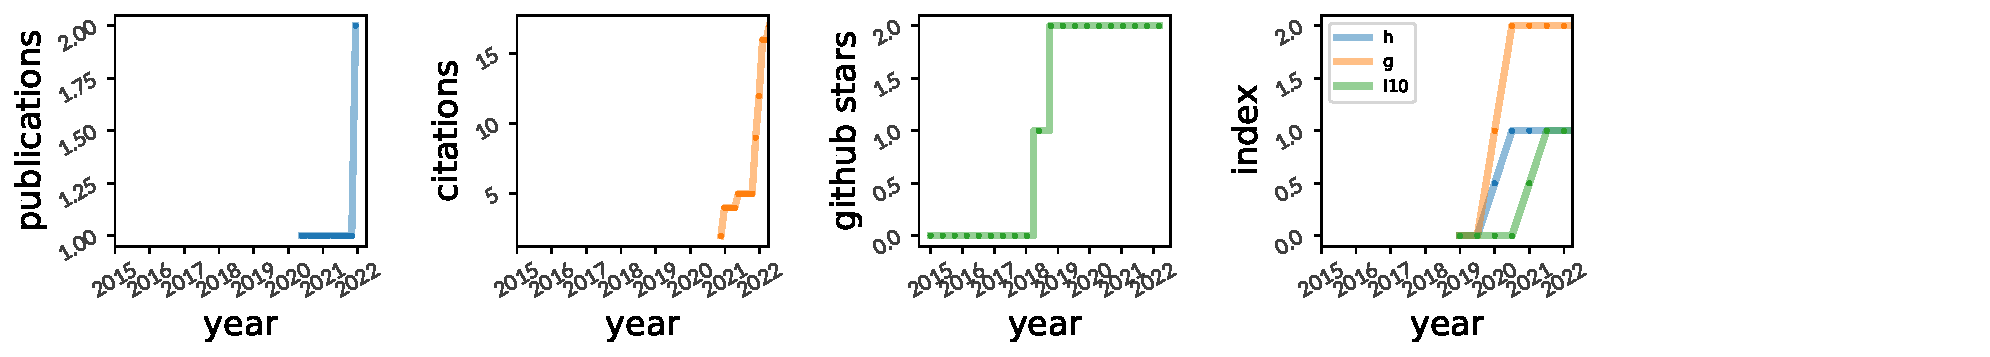
\includegraphics[height=1.25in]{metrics.pdf}
  %  }
  %  \pagebreak
%\fi
%\fi
%----------------------------------------------------------------------------------------
%	TEACHING
%----------------------------------------------------------------------------------------
%\ifdefined \onepage \else
%\aside{links}{0.05}{
%    {\color{numcolor}\faVideoCamera} \, \link{https://tinyurl.com/wnxmxb43}{LSST Lecture I}\\[0.5em]
%    {\color{numcolor}\faCloudDownload} \, \link{https://tinyurl.com/9247pj4}{LSST Worksheet I}\\[0.5em]
%    {\color{numcolor}\faVideoCamera} \, \link{https://drive.google.com/file/d/1PW-5Tkwnai7uQAZB4COFBUVTgWMZkE1P/view?usp=sharing}{LSST Lecture II}\\[0.5em]
%    {\color{numcolor}\faCloudDownload} \, \link{https://github.com/LSSTC-DSFP/LSSTC-DSFP-Sessions/tree/main/Session13/Day2}{LSST Worksheet II}\\[0.5em]
%}
%\fi

%\iffalse
\vspace{2.5cm}

\section{Software}

\begin{entrylist}
    %------------------------------------------------

    \entry
    {\textbf{star\_lifting}}
    {\link{https://github.com/mscoggs/star_lifting}{Repository}}
    {}
    {%
        \vspace{-1em}
        \begin{list}{{\color{numcolor}$-$}}{\cvlist}
            \item A MESA wrapper which evolves the star with a time-depedent mass loss rate, keeping flux on a habitable planet constant.
        \end{list}
    }
    %------------------------------------------------

    \entry
    {\textbf{qubit\_simulation}}
    {\link{https://github.com/mscoggs/qubit_simulation}{Repository}}
    {}
    {%
        \vspace{-1em}
        \begin{list}{{\color{numcolor}$-$}}{\cvlist}
            \item Simulating the evolution of a superconducting chip with the goal of finding patterns in the optimal protocols (values of the controls over time which evolve an initial state into a target state in the shortest possible time) over a variety of initial and target combinations.
        \end{list}
    }

    %------------------------------------------------

    \entry
    {\textbf{no\_wave\_qm}}
    {\link{https://github.com/mscoggs/no_wave_qm}{Repository}}
    {}
    {%
        \vspace{-1em}
        \begin{list}{{\color{numcolor}$-$}}{\cvlist}
            \item Simulating the evolution according to a hamilton-jacobi formulation of QM which replaces the wave with a configuration space density and equations of motion. Trajectory tracking using a 4-th order Runge Kutta technique.
        \end{list}
    }



\end{entrylist}
%\fi
%----------------------------------------------------------------------------------------
%	STUDENTS
%----------------------------------------------------------------------------------------
%\iffalse
\vspace{-0.5cm}



  \section{Outreach \& Press}
      \begin{entrylist}

          %------------------------------------------------

          \entry
          {2022}
          {\link{https://www.youtube.com/watch?v=IY0KWLanlLM&ab_channel=CoolWorlds}{Lazarus Stars - Extending Stellar Lifespans by Billions of Years}}
          {Youtube}

          %------------------------------------------------
          \entry
          {2023}
	      {\link{https://www.skyatnightmagazine.com/space-science/reducing-sun-mass-save-earth-in-the-future}{Could reducing the Sun's mass stop it destroying Earth in the future?}}
          {BBC Sky at Night}


          \entry
          {2023}
	      {\link{https://www.inverse.com/science/dyson-swarms-could-keep-aging-stars-from-burning-out}{Aliens Could Build Massive Megastructures to Save Dying Stars}}
          {Inverse}

          \entry
          {2022}
          {\link{https://github.com/mscoggs/intro_to_computational_astro}{Introduction to Computational Astronomy}}
          {Online}

      \end{entrylist}
      %------------------------------------------------



%\fi
%\iffalse
\section{Teaching \& Service}
\begin{entrylist}
\vspace{-0.3cm}


    \entry
    {2023}
    {Journal Reviewer: {\normalfont ApJ}} 
    {}
    {}
    %------------------------------------------------
    \entry
    {2023-}
	{Associate Director: {\normalfont Science Research Mentoring Program}}
    {Columbia University}
	{}
    %------------------------------------------------

    \entry
    {2021-2023}
    {Graduate Teaching Assistant}
    {Columbia University}
	{}

    %------------------------------------------------

    \entry
    {2020-2021}
    {Mathematics Teaching Assistant}
    {WWU}
	{}

    %------------------------------------------------

    \entry
    {2017-2020}
    {Physics Teaching Assistant}
    {WWU}
    {%
        \vspace{-1em}
        \begin{list}{{\color{numcolor}$-$}}{\cvlist}
            \item Responsible for facilitating/grading a section of the weekly lab for Physics w/ Calc 161-163, 220, and Tools and Data Analysis 322
        \end{list}
    }

    %------------------------------------------------

    \entry
    {2019}
    {Student Faculty Hiring Committee}
    {WWU}
	{}

    %------------------------------------------------

    \entry
    {2018-2019}
    {Physics Study Group Facilitator}
    {WWU}
    {%
        \vspace{-1em}
        \begin{list}{{\color{numcolor}$-$}}{\cvlist}
            \item Responsible for creating content and leading a 2 hour weekly study group for Physics w/ Calc 161-163
        \end{list}
    }

    %------------------------------------------------

    \entry
    {2018-2019}
    {Math Tutoring Fellow}
    {WWU}
    {%
        \vspace{-1em}
        \begin{list}{{\color{numcolor}$-$}}{\cvlist}
            \item Responsible for tutoring a majority of the undergraduate math classes, Calculus I up to Intro. to Abstract Algebra.
        \end{list}
    }


\end{entrylist}
%\fi
%STUDENTS


\vspace{0.3cm}

%\iffalse
  \section{Mentoring}
      \begin{entrylist}

	    \entry
	    {2023}
	      {Undergraduate Students} 
	      {}
	    {%
		\vspace{-1em}
		\begin{list}{{\color{numcolor}$-$}}{\cvlist}
		\item Andrea Dubbels - Abnormal Photometry in the GAIA DR3 Catalog (in prep)

		\end{list}
	    }
          %------------------------------------------------
	    \entry
	    {2023}
	      {High School Students} 
	      {}
	    {%
		\vspace{-1em}
		\begin{list}{{\color{numcolor}$-$}}{\cvlist}
		\item Students took part in 2-12 month projects designed to expose them to astrophysics and research skills. Some projects have been (or will be) submitted to high school journals.
		    \item Junhao Lei - A review of dark matter (accepted, International Journal of High School Research)
		    \item Iulia Achim - Exploring the potential for habitability around a black hole (under review, Journal of Emerging Investigators)
		    \item Estefania Olaiz - A new triple star system (in prep).
		    \item Pratham Aggarwal - The origins of supermassive black holes (in prep)
		    \item Jiarui Shi - Could Earth's transit be detected by known exoplanets? (in prep)
		    \item Hiep Duc Nguyen - "missing mass" and the need for dark matter
		    \item Jai Nair - The search for biosignatures
		    \item Weibo Qin - Do astrological signs correlate with personality? 
		    \item Elenes Diana - A review of black hole vs. host galaxy relations
		    \item William Li - Using ML to predict Solar Cycles

		\end{list}
	    }
          %------------------------------------------------


      \end{entrylist}
      %------------------------------------------------

      \vspace{-1cm}


%\fi

\iffalse
    \aside{}{4.2}{
    {\footnotesize primary developer}\\[1em]
    \hrule
    {\footnotesize secondary developer}
    }
\fi

\iffalse
    \section{Computing Experience}

    \begin{entrylist}

        %------------------------------------------------

        \entry
        {\textbf{Languages}(years): }
        {\textnormal{  \ C++(4), Python(4), C(3), Java(1), Matlab(1), Wolfram(1), Scheme(0.5), SQL(0.5)}}
        {}
        {
        }

        %------------------------------------------------
        \entry
        {\textbf{OS}: }
        {\textnormal{ \ Linux, mostly Ubuntu (5),  \   Windows (10+) \  Mac OS X (1)}}
        {}
        {
        }

        %------------------------------------------------
        \entry
        {\textbf{HPC Experience}: }
        {\textnormal{ WWU's CSCI Cluster \& CSE Cluster (Over 250 CPU years), Stampede2 (ongoing}}
        {}
        {
        }


    \end{entrylist}
\fi



%----------------------------------------------------------------------------------------
%	STATS
%----------------------------------------------------------------------------------------
%\iffalse

\vspace{0.5cm}
\aside{stats}{0.075}{
    \vspace*{0.5em}
    \input{pubs_summary}
}
%\fi


%----------------------------------------------------------------------------------------
%	PUBLICATIONS
%----------------------------------------------------------------------------------------


\ifdefined \withpubs
    %
    \ifdefined \citationskip
    \else
        \def\citationskip{0.95}
    \fi
    %\aside{}{\citationskip}{
    %{\footnotesize citations $\longrightarrow$}\\[0em]
    %{\footnotesize (refereed in \textbf{bold})}
    %}
    %
    \section{Publications}
    %
    \begin{list}{}{\pubslist}
        \input{pubs}
    \end{list}
    %
    \vspace{1em}
\fi

%----------------------------------------------------------------------------------------
%	TALKS
%----------------------------------------------------------------------------------------

\vspace{-0.5cm}

\ifdefined \withtalks

    \section{Selected Talks}
    %
    \vspace{-0.3cm}

    \begin{list}{}{\pubslist}
        \input{talks}
    \end{list}
\fi

\end{document}
